\documentclass[10pt]{amsart}

\usepackage{algorithm}
\usepackage[noend]{algpseudocode}
\usepackage{amsfonts}
\usepackage{amsmath}
\usepackage{amssymb}
\usepackage{amsthm}
\usepackage[backend=biber, citestyle=numeric-comp, bibstyle=ieee]{biblatex}
\usepackage{cancel}
\usepackage{changepage}
\usepackage{enumitem}
\usepackage{fancyhdr}
\usepackage{fontspec}
\usepackage{fullpage}
\usepackage[hidelinks]{hyperref}
\usepackage{longtable}
\usepackage{mathtools}
\usepackage{physics}
\usepackage[skins]{tcolorbox}
\usepackage{thmtools}
\usepackage{tikz}
\usepackage{tikz-3dplot}
\usetikzlibrary{angles, cd, quantikz, quotes, patterns}
\usepackage{titlesec}
\usepackage[normalem]{ulem}
\usepackage{wasysym}

\usepackage{tikz-cd}

\usepackage{bookmark}
\usepackage[nameinlink]{cleveref}

\titleformat{\section}[runin]{\normalsize\bfseries}{\thesection}{1em}{}[]
\titleformat{\subsection}[runin]{\normalsize\bfseries}{\thesubsection}{1em}{}[]
\titleformat{\subsubsection}[runin]{\normalsize\bfseries}{\thesubsubsection}{1em}{}[]

\addbibresource{zeno_effect.bib}

\theoremstyle{definition}
\newtheorem{theorem}{Theorem}
\newtheorem{definition}{Definition}
\theoremstyle{remark}
\newtheorem{problem}[theorem]{Problem}
\newtheorem{lemma}[theorem]{Lemma}
\newtheorem{remark}[theorem]{Remark}
\newtheorem{observation}[theorem]{Observation}
\newtheorem{example}[theorem]{Example}
\newtheorem{corollary}[theorem]{Corollary}

\renewcommand{\qedsymbol}{\(\blacksquare\)}

\setlength{\parindent}{0pt}

\DeclareMathOperator{\controrot}{CR}
\DeclareMathOperator{\expectation}{E}
\DeclareMathOperator{\gf}{GF}
\DeclareMathOperator{\qft}{QFT}
\DeclareMathOperator{\rk}{rk}
\DeclareMathOperator{\defect}{def}
\DeclareMathOperator{\swapgate}{SWAP}
\DeclareMathOperator{\che}{CHE}
\DeclareMathOperator{\poly}{poly}
\DeclareMathOperator{\Span}{Span}
\DeclareMathOperator{\diag}{diag}

\newcommand{\djk}{\delta_{j, k}}
\newcommand{\tlk}{\tilde{\lambda_k}}

\newcommand{\evalat}[2]{\left.{#1}\middle|\right._{#2}}

% SOURCE: https://tex.stackexchange.com/questions/296151/double-head-and-hook-arrow
\newcommand{\hookdoubleheadrightarrow}{%
  \hookrightarrow\mathrel{\mspace{-15mu}}\rightarrow
}

\newcommand{\draftcomment}[2]{\textcolor{#1}{#2}}

\newtcolorbox{simpleframebox}{enhanced, colback=white, halign=center, frame code={%
\draw[very thin] (frame.north west) -- (frame.north east) -- (frame.south east) -- (frame.south west) -- (frame.north west);
}}

\begin{document}
    \section*{The Zeno Effect for Quantum Computation} \hfill valentinpi, Last Change: August 29, 2023

    The following notes discuss the so-called \emph{Quantum Zeno Effect} (QZE) in the context of Quantum Computing. We use \cite{Misra_1977} as our main source, a useful exercise for the topic can be found in \cite[pp. 442-443]{Griffiths}.

    To explain this phenomenon, we consider the framework of \emph{undecayed} and \emph{decayed} states given in the article by Misra and Sudarshan \cite[p. 756]{Misra_1977}. Let \(n \in \mathbb{N}_{\geq 1}\), \(N \coloneqq 2^n\), \(U(N) \coloneqq \{U \in \mathbb{C}^{N \times N} \mid U \text{ unitär}\}\), \(H(N) \coloneqq \{H \in \mathbb{C}^{N \times N} \mid H \text{ Hamiltonian}\}\) and \(S(\mathbb{C}^N) \coloneqq \{\ket{\psi} \in \mathbb{C}^N \mid \norm{\ket{\psi}} = 1\}\), the latter two for \(n\) loose. Consider an \(n\)-Qubit quantum register in any initial state \(\ket{\Psi_0} \in S(\mathbb{C}^N)\). Suppose the register evolves along a unitary path \(U(t) \coloneqq e^{iHt} \in U(N)\), \(H \in H(N)\), \(t \in \mathbb{R}\). Recall especially, that \((\mathbb{R}, +) \to (U(N), \cdot), t \mapsto e^{iHt}\) is a group homomorphism. Also let \(\mathcal{M} \in \mathbb{C}^{N \times N}\) be an orthogonal projector into a subspace of \(\mathbb{C}^N\). We now suppose \(\ket{\Psi_0} \in \Im(\mathcal{M})\) and that in a timeframe \([0, t]\) with \(t \in \mathbb{R}_{> 0}\) fixed, the system may spontaneously \emph{decay}, undergoing a state change from a state in \(D \coloneqq \Im(\mathcal{M}) \cap S(\mathbb{C}^N)\), the space of \emph{undecayed} states, into a state from \(D^\perp\), defined analogously, the space of \emph{decayed} states. Thus, the system initially starts out undecayed. We denote decayed states with an additional asterix, like for instance \(\ket{\Psi_0'}\) in the following drawing.

    \begin{figure}[!hbtp]
        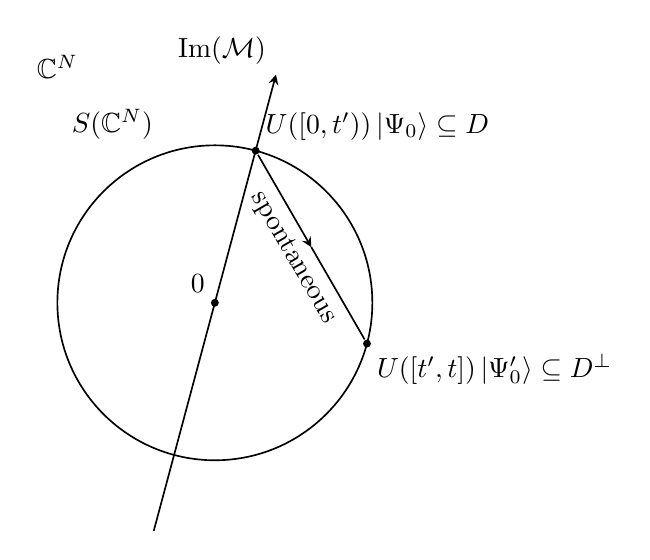
\begin{tikzpicture}[>=stealth, semithick]
            \tikzset{
                point/.style={circle, fill, inner sep=0pt, minimum size=1mm}
            };
            \node at (-2, 3) {\(\mathbb{C}^N\)};
            \node[point] (0) at (0, 0) {};
            \node[above left] at (0) {\(0\)};
            \draw (0, 0) circle (2cm);
            \draw[->] ($1.5*(255:2cm)$) -- ($1.5*(75:2cm)$) node [above left] {\(\Im(\mathcal{M})\)};
            \node[point] (1) at (75:2cm) {};
            \node[above right] at (1) {\(U([0, t'))\ket{\Psi_0} \subseteq D\)};
            \node[point] (2) at (-15:2cm) {};
            \node[below right] at (2) {\(U([t', t])\ket{\Psi_0'} \subseteq D^\perp\)};
            %\draw[line width=0.66mm] (2) arc (-15:30:2);
            %\draw[line width=0.66mm] (2) arc (-15:-30:2);
            \draw[->] (1) -- ($(1)!0.5!(2)$) node[below, rotate=-60] {spontaneous};
            \draw ($(1)!0.5!(2)$) -- (2);
            \node[above right] at (135:2.75cm) {\(S(\mathbb{C}^N)\)};
        \end{tikzpicture}
    \end{figure}

    Consider especially, that we can interpret a contribution of the orthogonal subspace due to a unitary transformation as a spontaneous decay in the sense that part of the state becomes decayed. The statement of the Zeno paradox is now, that if we perform very fast subsequent measurements on the system, while the unitary evolution is taking place, the system practically cannot evolve, or shorter:
    \begin{simpleframebox}
        Under continuous measurement, a quantum system will never decay.
    \end{simpleframebox}
    Four remarks: (a) The name of the effect is based on the paradox by the Greek philosopher Zeno, where a moving arrow is denied the possibility of motion, because one can look at arbitrary small time intervals of movement, effectively erasing the motion\footnote{There are more Zeno paradoxes, including an ancient formulation of interval nestings, see the \hyperref[appendix]{Appendix}.} \cite[p. 757]{Misra_1977}. (b) The effect is not to be confused with the \emph{Quantum Zeeman Effect}, where energy levels are shifted by magnetic fields (possibly interesting for adiabatic quantum computation) \cite[pp. 304-305]{Griffiths}. (c) Whilst it is not the same concept, the statement somewhat continues the Heisenberg uncertainty principle \cite[pp. 19-20]{Griffiths}, although the statements are completely different. (d) We discuss a rigorous formulation in the following, which is only valid for idealized closed quantum systems, more general versions have been developed in the meantime \cite{Chiu_1977}.

    \section*{Outline of the Rigorous Formulation} The rigorous formulation of the Zeno effect \cite[p. 759]{Tavakoli} requires more preliminaries and a refresher in regards to density matrices, or an alternative formulation in the states-as-vector setting\footnote{..., which to my knowledge has not been done yet, ...}, but we will outline the mathematical formulation here.
    %For simplicity, assume that the orthogonal projection \(\mathcal{M}\) is a binary-valued diagonal matrix, this is wlog., as these equations with some omitted equations behave the same in general. Then the success probability of measuring wrt. the subspace \(D\) at time point \(t\) is given by
    %\begin{align}
    %    \sum_{\ket{i} \in D} |a_i|^2 = a^\dagger \mathcal{M} a = \tr(\bra{\Psi_0}U^\dagger(t)\mathcal{M}U\ket{\Psi_0})
    %\end{align}
    %with \(a \coloneqq (a_i)_{i \in [0, N-1]_{\mathbb{N}}} \coloneqq U(t)\ket{\Psi_0}\). Analogously, the probability of failure is \(\tr(\bra{\Psi_0}U^\dagger(t)(E_N-\mathcal{M})U\ket{\Psi_0})\).
    Let \(\ket{\Psi(m, t)}\) for \(m \in \mathbb{N}_{\geq 1}\) be the state of the system after evolving for a time \(t \in \mathbb{R}_{> 0}\) and in the meantime performing \(m+1\) subsequent measurements at the time points \([0, m]_{\mathbb{N}} \cdot t/m\), if the system does not decay in the meantime. The change of states thus takes on the following form
    \newcommand{\measurementsymbol}{
        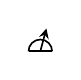
\begin{tikzpicture}[>=stealth, semithick, scale=1.5]
            \draw (-0.1, 0) -- (0.1, 0);
            \draw (0.1, 0) arc (0:180:0.1);
            \draw[->] (0, 0) -- (75:0.2);
        \end{tikzpicture}
    }
    \begin{align}
        \ket{\Psi_0} \xmapsto{\measurementsymbol} \ket{\Psi_0} \mapsto U(t/m)\ket{\Psi_0} \xmapsto{\measurementsymbol} \frac{1}{\norm{\mathcal{M}U(t/m)\ket{\Psi_0}}} \mathcal{M}U(t/m)\ket{\Psi_0} = \ket{\Psi(1, t/m)} \mapsto ... \mapsto \ket{\Psi(m, t)}
    \end{align}
    This gives the general idea for the following framework: Using density matrices \cite[pp. 98-101]{Nielsen}, we can express the same relation more elegantly in the form
    \begin{align}
        \rho(m, t) = T_m(t) \rho T_m^*(t) \text{ with } T_m(t) \coloneqq (\mathcal{M}U(t/m)\mathcal{M})^m
    \end{align}
    where \(\rho \in \mathbb{C}^{N \times N}\) is the density operator of the initial state and \(\rho(m, t)\) the density operator representation of \(\ket{\Psi(m, t)}\). Under certain formal conditions, the strong limit operator \(\lim_{m \to \infty} T_m(t) \eqqcolon T(t)\) exists with the properties (a) that it can be continuously extended to \(T(0) = \mathcal{M}\) (b) \(T(s+s')=T(s)+T(s')\) (c) \(T^*(s) = T(-s)\) for any \(s, s' \in \mathbb{R}\), implying \(T^*(t)T(t)=\mathcal{M}\). It can also be shown that the probability of the system to \emph{not} decay at some point in \([0, t]\) is given by
    \begin{align}
        \tr(\rho T^*(t)T(t))
    \end{align}
    implying no decay with the properties of \(T\).


    \begin{figure}[!hbtp]
        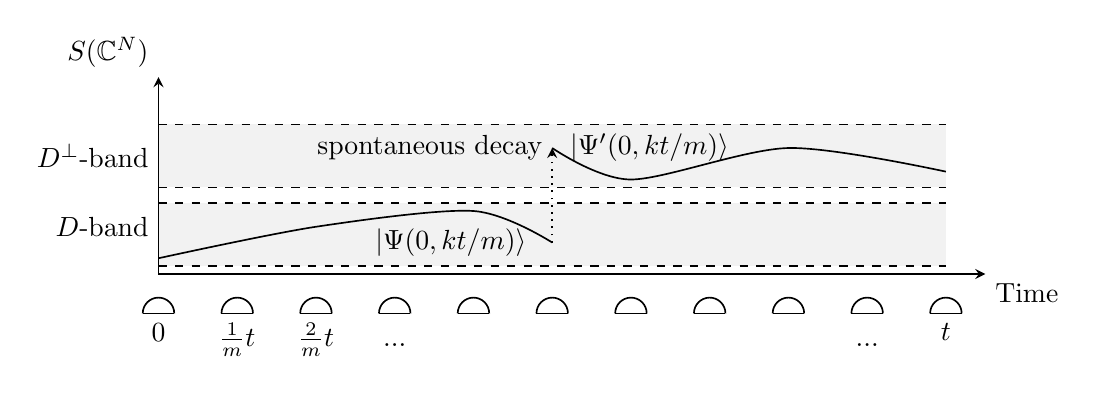
\begin{tikzpicture}[>=stealth, semithick, scale=2]
            \def\w{5};
            \def\n{10};
            \fill[gray!10] (0, 0.05) rectangle (\w, 0.45);
            \draw[dashed] (0, 0.05) -- (\w, 0.05);
            \draw[dashed] (0, 0.45) -- (\w, 0.45);
            \node[above left] at (0, 1.25) {\(S(\mathbb{C}^N)\)};
            \fill[gray!10] (0, 0.55) rectangle (\w, 0.95);
            \draw[dashed] (0, 0.55) -- (\w, 0.55);
            \draw[dashed] (0, 0.95) -- (\w, 0.95);
            \draw[->] (0, 0) -- (\w+0.25, 0) node[below right] {Time};
            \draw[->] (0, 0) -- (0, 1.25);
            \foreach \x in {0, 1, ..., \n}{
                \draw (\w*\x/\n-0.1, -0.25) -- (\w*\x/\n+0.1, -0.25);
                \draw (\w*\x/\n+0.1, -0.25) arc (0:180:0.1);
            }
            \node[below] at (\w*0/\n, -0.25) {\(0\)};
            \node[below] at (\w*1/\n, -0.25) {\(\frac{1}{m}t\)};
            \node[below] at (\w*2/\n, -0.25) {\(\frac{2}{m}t\)};
            \node[below=0.25cm] at (\w*3/\n, -0.25) {\(...\)};
            \node[below=0.25cm] at (\w*9/\n, -0.25) {\(...\)};
            \node[below] at (\w*10/\n, -0.25) {\(t\)};
            \draw plot[looseness=0.5, smooth] coordinates { (0, 0.1) (1, 0.3) (2, 0.4) (2.5, 0.2) };
            \draw plot[looseness=0.5, smooth] coordinates { (2.5, 0.8) (3, 0.6) (4, 0.8) (5, 0.65) };
            \draw[->, dotted] (2.5, 0.2) -- (2.5, 0.8) node[left] {spontaneous decay};
            \node[left] at (0, 0.3) {\(D\)-band};
            \node[left] at (0, 0.75) {\(D^\perp\)-band};
            \node[left=2mm] at (2.5, 0.2) {\(\ket{\Psi(0, kt/m)}\)};
            \node[right=1mm] at (2.5, 0.8) {\(\ket{\Psi'(0, kt/m)}\)};
        \end{tikzpicture}
    \end{figure}
    \begin{figure}[!hbtp]
        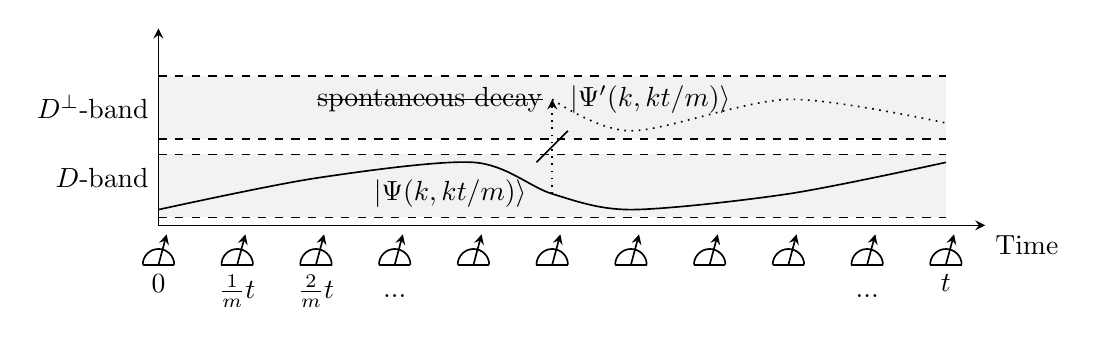
\begin{tikzpicture}[>=stealth, semithick, scale=2]
            \def\w{5};
            \def\n{10};
            \fill[gray!10] (0, 0.05) rectangle (\w, 0.45);
            \draw[dashed] (0, 0.05) -- (\w, 0.05);
            \draw[dashed] (0, 0.45) -- (\w, 0.45);
            \fill[gray!10] (0, 0.55) rectangle (\w, 0.95);
            \draw[dashed] (0, 0.55) -- (\w, 0.55);
            \draw[dashed] (0, 0.95) -- (\w, 0.95);
            \draw[->] (0, 0) -- (\w+0.25, 0) node[below right] {Time};
            \draw[->] (0, 0) -- (0, 1.25);
            \foreach \x in {0, 1, ..., \n}{
                \draw (\w*\x/\n-0.1, -0.25) -- (\w*\x/\n+0.1, -0.25);
                \draw (\w*\x/\n+0.1, -0.25) arc (0:180:0.1);
                \draw[->] (\w*\x/\n, -0.25) -- ($(\w*\x/\n, -0.25)+(75:0.2)$);
            }
            \node[below] at (\w*0/\n, -0.25) {\(0\)};
            \node[below] at (\w*1/\n, -0.25) {\(\frac{1}{m}t\)};
            \node[below] at (\w*2/\n, -0.25) {\(\frac{2}{m}t\)};
            \node[below=0.25cm] at (\w*3/\n, -0.25) {\(...\)};
            \node[below=0.25cm] at (\w*9/\n, -0.25) {\(...\)};
            \node[below] at (\w*10/\n, -0.25) {\(t\)};
            \draw plot[looseness=0.5, smooth] coordinates { (0, 0.1) (1, 0.3) (2, 0.4) (2.5, 0.2) (3, 0.1) (4, 0.2) (5, 0.4) };
            \draw[dotted] plot[looseness=0.5, smooth] coordinates { (2.5, 0.8) (3, 0.6) (4, 0.8) (5, 0.65) };
            \draw[->, dotted] (2.5, 0.2) -- (2.5, 0.8) node[left] {\sout{spontaneous decay}};
            \node[left] at (0, 0.3) {\(D\)-band};
            \node[left] at (0, 0.75) {\(D^\perp\)-band};
            \draw (2.5-0.1, 0.5-0.1) -- (2.5+0.1, 0.5+0.1);
            \node[left=2mm] at (2.5, 0.2) {\(\ket{\Psi(k, kt/m)}\)};
            \node[right=1mm] at (2.5, 0.8) {\(\ket{\Psi'(k, kt/m)}\)};
        \end{tikzpicture}
    \end{figure}

    \textbf{Possible Application in Quantum Algorithms} Adding to some recent publications using the Zeno effect in the field of quantum communication theory \cite{Hardy_1999, Tavakoli}, we may think of some more general applications of this effect in quantum algorithms. One idea may be to extract result qubits from a quantum computation.

    \phantom{}

    One idea may be the following. Suppose \(U \in U(N)\) is a quantum algorithm with an action \(\ket{0}^{\otimes n} \mapsto \bigotimes_{i=1}^n \ket{\psi_i}\). If we consider an \(n\)-qubit register as a tensor network of \(n\) single qubits, then for a fixed \(k \in [1, n]_{\mathbb{N}}\), we could possibly implement the projection to the \(k\)th qubit of the action of \(U\), designated as \(U_k\) with \(\ket{0}^{\otimes n} \mapsto \ket{0}^{k-1}\ket{\psi_k}\ket{0}^{n-k}\), using the Zeno effect, by continuously measuring wrt. the observable \(\{\Span(\{\bigotimes_{i=1}^{k-1}\ket{\xi_i} \otimes \ket{\xi_k} \otimes \bigotimes_{i=k+1}^n\ket{\xi_i} \mid \xi_k \in \{0, 1\}\}) \mid (\xi_1,...,\xi_{k-1},\xi_{k+1},...,\xi_n) \in \{0, 1\}^{n-1}\}\), whilst at the same time applying \(U\). In principle, we could vary the assumption to only allow for the non-entanglement of the \(k\)-th qubit or adjust the algorithm to allow for the evolution of multiple selected, different qubits.
    
    %\begin{figure}[!hbtp]
    %    \centering
    %    \begin{quantikz}
    %        \lstick{\(\ket{0}^{\otimes m}\)}    \qw & \gate{\text{QFT}_M} \qw & \gate[wires=2]{\Lambda_M(U)} \qw & \gate{\text{QFT}_M^\dagger} \qw & \meter{\(k\)}\\
    %        \lstick{\(\ket{\psi}\)}             \qw & \qw &                         \qw
    %    \end{quantikz}
    %\end{figure}

    \begin{figure}[!hbtp]
        \centering
        \begin{quantikz}[thin lines]
            \lstick{\(\ket{0}^{\otimes (k-1)}\)} \qw & \meter{} \gategroup[3, steps=4, style={fill=white, inner sep=6pt}, background]{\(U = U(t_1)\)} \qw & \meter{} \qw & \gate[style={draw=none}]{...} \qw & \meter{} \qw & \rstick{\(\ket{0}^{\otimes (k-1)}\)} \qw\\
            \lstick{\(\ket{0}\)}                 \qw & \gate{U_k(t)} \qw & \gate{U_k(t)} \qw & \gate[style={draw=none}]{...} & \gate{U_k(t)} \qw & \rstick{\(\ket{\psi_k}\)} \qw\\
            \lstick{\(\ket{0}^{\otimes (n-k)}\)} \qw & \meter{} \qw & \meter{} \qw & \gate[style={draw=none}]{...} \qw & \meter{} \qw & \rstick{\(\ket{0}^{\otimes (n-k)}\)} \qw
        \end{quantikz}
    \end{figure}

    An investigation of the precise quantum physics of the Zeno effect may be necessary to confirm this, however, some other authors have also already proposed the use of the Zeno effect in this way \cite[p. 4]{Wan}, but it has never so far been treated in a general way as a part of a quantum-algorithmic toolbox:
    \begin{quote}
        "The concept of the quantum Zeno effect allows the total Hilbert space to be divided into Zeno subspaces, and different components of the density matrix can independently evolve within each sector."
    \end{quote}

    \section*{Appendix: The Zeno Paradox} \label{appendix} The main source for the paradox is Aristotles Physics, the necessary adjusted excerpt is taken from \cite[p. 110]{Aristotle}.

    \begin{quote}
        The third is [...] that the flying arrow is at rest, which result follows from the assumption that time is composed of moments [...]. he says that if everything when it occupies an equal space is at rest, and if that which is in locomotion is always in a now, the flying arrow is therefore motionless.
    \end{quote}


    \printbibliography{}
\end{document}
